\documentclass[dvipsnames, tikz]{standalone}

\usepackage{tikz}
\usetikzlibrary{tikzmark}
\usepackage{xcolor}
\usetikzlibrary{calc}

\begin{document}
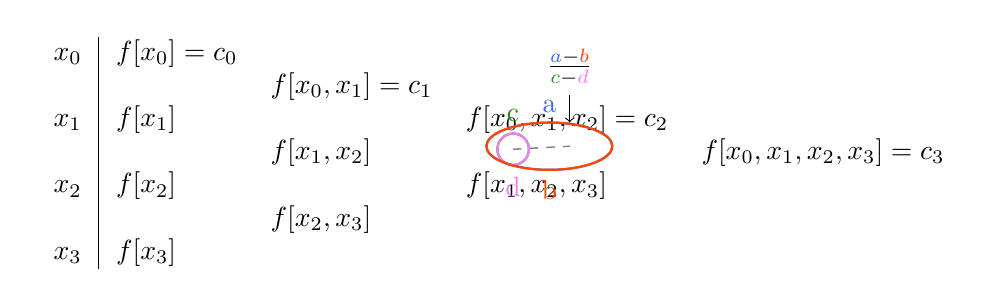
\begin{tikzpicture}[remember picture]
\node at (0,0) {\begin{tabular}{c|llll}
\subnode{C}{$x_0$} & $f[x_0]=c_0$\\
 & & $\subnode{A}{f[x_0,x_1]}=c_1$\\
$x_1$ & $f[x_1]$ & &$\subnode{E}{f[x_0,x_1,x_2]}=c_2$\\
 & & $\subnode{B}{f[x_1,x_2]}$ & & $f[x_0,x_1,x_2,x_3]=c_3$\\
\subnode{D}{$x_2$} & $f[x_2]$ & &$f[x_1,x_2,x_3]$\\
 & & $f[x_2,x_3]$\\
$x_3$ & $f[x_3]$\\
\end{tabular}};

\draw[dashed,gray] (D.center) -- (E.center);
\draw[dashed,gray] (C.center) -- (E.center);

\node[circle,thick,ForestGreen,draw, minimum size=4mm] at (C) {};
\node[anchor=south, ForestGreen] at (C.north) {c};
\node[circle,thick,Violet,draw, minimum size=4mm] at (D) {};
\node[anchor=north, Violet] at (D.south) {d};

\draw[thick,RoyalBlue] (A) ellipse (0.8cm and 0.3cm) node[above,yshift=3mm] {a};
\draw[thick,OrangeRed] (B) ellipse (0.8cm and 0.3cm) node[below,yshift=-3mm] {b};

\node (F) at ($(E)+(0,1cm)$) {$\frac{\textcolor{RoyalBlue}{a}-\textcolor{OrangeRed}{b}}{\textcolor{ForestGreen}{c}-\textcolor{Violet}{d}}$};

\draw[->] (F) -- (E);




\end{tikzpicture}
\end{document}